\documentclass[main]{subfiles}
\begin{document}

%@@@@@@@@@@@@@@@@@@@@@@@@@@@@@@
% Main Topics: revised simplex algorithm and degeneracy and anti-cycling rules
% The Simplex Algorithm III - 23.10.2017
% author: Vanessa Leite

\section{Simplex Algorithm III}

\subsection{The worst-case running time of a simplex algorithm}
Assumption: we select a pivot-column $j \in N$ with the maximal absolute value
of reduced cost.

\paragraph{Theorem: Klee-Minty Cube (KMC)} Under the previous assumption, the
simplex algorithm can take "exponentially" (related with the input size) many
steps.

\subparagraph{Proof (construction/deformation of the cube): }

$\mathcal{P} = \{x \in \mathbb{R}^n \mid Ax \leq b \}$ is a deformation of the
cube.

\begin{figure}[!h]
  \label{fig:projection}
  \caption{Cube degeneracy: skip one vertice. It can be seen as a "cube", but
  the skipped vertex is not part of the problem.}
  \centering
    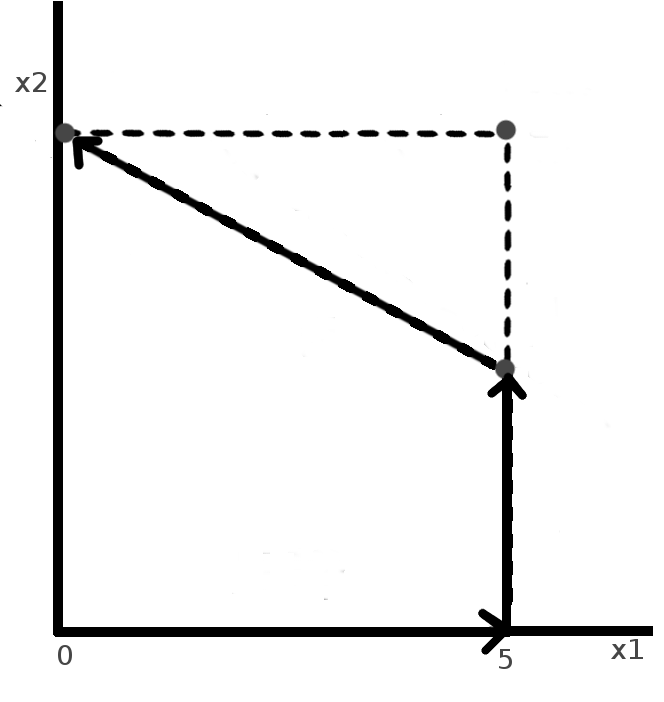
\includegraphics[width=0.2\textwidth]{imgs/kmc.png}
\end{figure}

\begin{equation*}
\begin{aligned}
& \max
& & 2x_1 + x_2 \\
& \text{subject to}
& & x_{1} \leq 5 \\
&&& 4x_1 + x_2 \leq 25\\
&&& x_1, x_2 \geq 0
\end{aligned}
\end{equation*}

$\rightarrow$ by adding slack variables:

\begin{equation*}
\begin{aligned}
& \max
& & 2x_1 + x_2 \\
& \text{subject to}
& & x_{1} + z_1 = 5 \\
&&& 4x_1 + x_2 + z_2 = 25\\
&&& x, z \geq 0
\end{aligned}
\end{equation*}

$\rightarrow \{z_1, z_2\}$ are the basis.\\

Pivot column $\{1\}$ (original vertex $(0,0)$. In the columnm $\{1\}$ the
maximum quantity is $x_1 = 5 - z_1$. Change the value of $x_1$ on the objective
function and constraints. We can ignore positive constants on the objective
function, they are irrelevant for maximization.

\begin{equation*}
\begin{aligned}
& \max
& & x_2 - 2z_1 \\
& \text{subject to}
& & x_{1} + z_1 = 5 \\
&&& -4z_1 + x_2 + z_2 = 5\\
&&& x, z \geq 0
\end{aligned}
\end{equation*}

$\rightarrow \{x_1, z_2\}$ are the basis, original vertex $(5,0)$, new pivot
column is $\{2\}$. We choose by trying to eliminate positive costs.\\
$x_2 = 5 - z_2 + 4z_1$

\begin{equation*}
\begin{aligned}
& \max
& & -z_2 + 2z_1 \\
& \text{subject to}
& & x_{1} + z_1 = 5 \\
&&& x_2 + z_2 -4z_1 = 5\\
&&& x, z \geq 0
\end{aligned}
\end{equation*}

$\rightarrow \{x_1, x_2\}$ are the basis, original vertex $(5,5)$.\\
$z_1 = 5 - x_1$

\begin{equation*}
\begin{aligned}
& \max
& & -z_2 - 2x_1 \\
& \text{subject to}
& & x_{1} + z_1 = 5 \\
&&& x_2 + z_2 +4x_1 = 25\\
&&& x, z \geq 0
\end{aligned}
\end{equation*}

$\rightarrow \{z_1, x_2\}$ are the basis, original solution $(0,25)$.
There is no positive costs in the objective function.\\

\subsubsection{The generalization}

Add $z$ as slack variables and turn inequalities in equalities.

\begin{equation*}
\begin{aligned}
& \max
& & 2^{n-1}x_1 + \dots + x_n \\
& \text{subject to}
& & z_1 + x_1 \leq (=) 5 \\
&&& z_2 + 4x_1 + x_2 \leq (=) 5 \times 5\\
&&& \vdots + 8x_1 + 4x_2 + x_3 \leq (=) 5 \times 5 \times 5\\
&&& \vdots + \vdots \leq (=) \vdots\\
&&& z_n + 2^n x_1 + 2^{n-2} x_2 + \dots + 2^2 x_{n-1} + x_n \leq (=) 5^n\\
&&& x, z \geq 0
\end{aligned}
\end{equation*}

The feasible region of this polyhedron is called the Klee-Mint Cube (KMC).

\paragraph{Observations:}
\begin{enumerate}
\item All basis of KMC are non-degenerate.
\item For any basis, either $x_i$ or $z_i$ is on the basis
\item The unique optimal solution is $x_1 = 0 = x_2 = \dots = x_{n-1}$;
$x_n = 5^n$ (maximum weight in the last variable).
\item Starting from zero and pivoting in a column with highest reduced cost
coefficient require $2^n - 1$ many pivoting steps.
\end{enumerate}

\subsection{Finding an initial basis}

\paragraph{Lemma: Let $\mathcal{P} = \{x \geq 0 \mid Ax = b\}$. By solving a
linear optimization problem, we can find an initial bfs if it exists or prove
that it does not exist.}

\subparagraph{Proof:}
First multiply every row by $-1$ if $b_i < 0$. Then, wlog $b \geq 0$.
Consider auxiliar system: $\alpha = \min \sum_{i=1}^{m} y_i$ st $ Ax + Iy = b$,
$x \geq 0$, $y \geq 0$. This system has a bfs, because the initial basis is
$x = 0$, $y = b$. A lower bound for $\alpha$ is zero, otherwise, there is no
bfs. If $\alpha > 0$, then no solution exists. If $\alpha = 0$ the SA
terminates with a basic solution only using $x$ variables.

\subsection{The Dual Simplex Algorithm}

Consider $\max \{y^T b \mid A^T y \leq c \}$ as the dual. Let $y^*$ be the dual
bfs associated with some basis $B \subseteq \{1, \dots, m\}$. Such bfs has the
property: $y^* = c^T_B A^{-1}_B$, and dual feasible implies $\bar{c} \geq 0$.

\paragraph{Lemma: Suppose $\exists i \in B$ st $\bar{b_i} < 0$:}
\begin{itemize}
\item We look into the matrix $A$, if $\bar{A_{ij}} \geq 0$ $\forall j \in N$
then $\displaystyle \max_{y \in \mathcal{D}} y^{T} b = + \infty$
\item Otherwise, $\lambda^* = \min \{\frac{-\bar{c_j}}{\bar{A_{ij}}} \mid
\bar{A_{ij}} < 0$, $j \in N \}$ and $(y^*)^T = (y^*)^T - \lambda^*
(A^{-1}_B)_i$ is feasible for the dual. $b^T y = b^T y^* - \lambda^*
\bar{b_j}$, i.e, $b^T y > b^T y^*$, where $\lambda^* = \frac{-\bar{c_k}}
{\bar{A_{ik}}}$ ($k$ is not in the basis).\\
$B \setminus \{i\} \cup \{k\}$ is a new basis.
\end{itemize}

\subparagraph{Proof:}
Let $y^T = (y^*)^T - \lambda (A^{-1}_B)_i$ where $\lambda > 0$.
$y^T A = (y^*)^T  A - \underbrace{\lambda}_{\geq 0}
\underbrace{\bar{A_i}}_{\geq 0} \leq c^T$.
In the otherwise case: $y^T A = (y^*)^T  A - \lambda^* A_i$. If $\bar{A_{ij}}
\geq 0 \rightarrow y^T A \leq c_j$, otherwise, if $\bar{A_{ij}} < 0 \rightarrow
y^T A \leq (y^*)^T A_{\cdot j} \frac{-\bar{c_j}}{-\bar{A_{ij}}} \bar{A_{ij}} =
\underbrace{c^T_B A^{-1}_B A_{\cdot j}}_{y^*} +
\underbrace{c_j - c^T_B A^{-1}_B A_{\cdot j}}_{\bar{c_j}} = c_j$.
$B\setminus \{i\} \cup \{k\}$ being a basis is the same argument as in lecture
8, pivoting-theorem.


\subsubsection{The major simplex steps in the dual setting}
\begin{enumerate}
\item Choose a dual bfs in the dual setting: $y^*$
\item $\bar{b} = A^{-1}_B b$
\item If $\bar{b} \geq 0$, stop: optimal
\item Otherwise, let $i \in B$, $\bar{b_i} < 0$
\subitem if $\bar{A_{ij}} \geq 0$ $\forall j \in N$, stop: unbounded
\subitem otherwise, compute $\lambda^* = min \{\frac{\bar{c_j}}{-\bar{A_{ij}}}
\mid \bar{A_{ij}} < 0$ $j \in N \}$ and an index $k \in N$, st $\lambda^* =
\frac{-\bar{c_k}}{\bar{A_{ik}}}$.
\item Swap indices and update solutions, $B = B\setminus \{i\} \cup \{k\}$, 
$(y^*)^T = (y^*)^T - \lambda^* (A^{-1}_B)_i$.
\end{enumerate}
\end{document}